\documentclass[conference]{IEEEtran}
\IEEEoverridecommandlockouts
% The preceding line is only needed to identify funding in the first footnote. If that is unneeded, please comment it out.
\usepackage{cite}
\usepackage{amsmath,amssymb,amsfonts}
\usepackage{algorithmic}
\usepackage{array}
\usepackage{booktabs}
\usepackage{graphicx}
\usepackage{subcaption}
\usepackage{textcomp}
\usepackage{xcolor}
\newcolumntype{L}[1]{>{\raggedright\arraybackslash}p{#1}}
\newcolumntype{C}[1]{>{\centering\arraybackslash}p{#1}}
\emergencystretch=2em
\def\BibTeX{{\rm B\kern-.05em{\sc i\kern-.025em b}\kern-.08em
T\kern-.1667em\lower.7ex\hbox{E}\kern-.125emX}}
\begin{document}

\title{Multi-Resolution Raster Visualization Using Semantic-Adaptive Hilbert (SAH) Indexing for Standalone and Distributed Display Systems}

\author{
  \IEEEauthorblockN{Bipasha Garg}
  \IEEEauthorblockA{\textit{Data Science \& Analytics Center}\\
    \textit{University}\\
    Email: bipasha.garg@research.iiit.ac.in}
  \and
  \IEEEauthorblockN{Tanish Gupta}
  \IEEEauthorblockA{\textit{Data Science \& Analytics Center}\\
    \textit{University}\\
    Email: tanish.gupta@research.iiit.ac.in}
}
\maketitle

% ── Abstract ──────────────────────────────────────────────────────────────────
\begin{abstract}
Traditional geospatial raster indexing systems treat all spatial regions with uniform computational budgets, resulting in severe inefficiency when processing heterogeneous landscapes that combine open water, transitional coastlines, and dense urban environments. This paper presents a system built on the \textit{Semantic-Adaptive Hilbert} (SAH) indexing architecture, which assigns variable index resolution according to the visual complexity of each tile. Using a two-factor classifier combining a pixel-level Water Score and Shannon Entropy, tiles are categorized into three semantic classes, Water, Coast, and Urban, each assigned a distinct Hilbert curve order (2, 3, and 4 respectively). A four-stage RAM-resident query engine eliminates disk I/O during query serving and achieves up to 99.9\% record pruning at fine zoom levels. The same backend serves both standalone React/Flask displays and distributed 8-panel SAGE2 walls without modification. Benchmark results demonstrate a peak speedup of $214.2\times$ over naive scanning and $O(\log N + K)$ query complexity versus $O(N)$ in legacy systems.
\end{abstract}

\begin{IEEEkeywords}
  spatial indexing, Hilbert curve, raster visualization, semantic segmentation, multi-resolution tiling, distributed display systems, geospatial computing
\end{IEEEkeywords}

% ── I. Introduction ───────────────────────────────────────────────────────────
\section{Introduction}

Geospatial raster datasets present a fundamental indexing challenge: the information density of spatial regions varies dramatically. A tile of open ocean contains negligible visual complexity, while an equivalent-area urban tile may encode thousands of meaningful structures. Despite this disparity, traditional spatial indexing approaches allocate identical computational resources to every tile through uniform grid decomposition.

This uniform treatment creates three compounding problems. First,
\textit{pre-mosaicking bottlenecks} require thousands of files to be stitched
before any query can execute, creating pipeline latencies exceeding 75 hours for 1{,}000-file datasets. Second, \textit{naïve row-major indexing} scatters spatially adjacent tiles across non-contiguous memory addresses, forcing sequential scans even for localized viewport queries. Third,
\textit{uniform tile depth} wastes storage and compute on featureless regions.

The system addresses all three problems through the Semantic-Adaptive Hilbert (SAH) indexing approach, which: (1) classifies tiles by visual complexity before assigning index depth; (2) uses a Hilbert space-filling curve to preserve spatial locality in one-dimensional key space; and (3) serves query results entirely from RAM with zero disk I/O after server startup.

% ── II. Problem Statement ─────────────────────────────────────────────────────
\section{Problem Statement}

The core inefficiency of legacy geospatial raster pipelines derives from the
\textit{uniformity assumption}: every tile in a dataset receives the same
quadtree depth, the same number of index records, and the same memory bandwidth budget, regardless of whether it covers open ocean or a dense city center. This produces three observable failure modes:

\textbf{Pre-Mosaicking Bottleneck.} Traditional pipelines require full dataset
mosaicking before the tile-pyramid stage can begin. For large collections of GeoTIFF files, this sequential dependency produces hours of idle CPU time and prevents incremental query serving.

\textbf{Scattered Memory Layout.} Row-major indexing maps 2D tile coordinates
to 1D keys by lexicographic ordering ($\text{row} \times \text{width} +
\text{col}$). This scheme places geographically adjacent tiles at numerically
distant array positions, degrading spatial range queries to full-table scans.

\textbf{Uniform Tile Waste.} Identical subdivision depth for all semantic
classes generates up to $16\times$ more index records per water tile than the data content justifies, inflating memory footprint and query scan cost proportionally.

% ── III. The SAH Architecture ─────────────────────────────────────────────────
\section{The SAH Architecture}

\subsection{Semantic Classification}

SAH classifies each base tile using two independent metrics computed directly from raw pixel channels.

\textbf{Water Score.} Defined per pixel as
\begin{equation}
  S_w = \frac{B - R}{R + G + B}
  \label{eq:waterscore}
\end{equation}
and averaged over the tile. Positive values indicate water; negative values indicate terrestrial surface. This metric exploits the spectral reflectance difference between water bodies (blue-dominant) and land covers (red/green-dominant).

\textbf{Shannon Entropy.} Pixel-level randomness
\begin{equation}
  H = -\sum_{x} p(x)\,\log_2 p(x)
  \label{eq:entropy}
\end{equation}
computed over the intensity histogram of the tile~\cite{bariviera2024texture}. Low entropy ($H < 1.0$) characterizes visually flat, featureless regions. High entropy ($H > 2.5$) characterizes informationally dense regions with high structural variation.

These two metrics jointly determine the semantic class assignment and associated Hilbert curve order, as shown in Table~\ref{tab:lod}.

\begin{table}[t]
  \caption{Semantic Class Assignments and Index Parameters}
  \label{tab:lod}
  \centering
  \scriptsize
  \renewcommand{\arraystretch}{1.1}
  \setlength{\tabcolsep}{3pt}
  \begin{tabular}{c l c c c}
    \toprule
    \textbf{Class} & \textbf{Condition} & \textbf{Order} &
    \textbf{Grid} & \textbf{Records} \\
    \midrule
    Water & $S_w>0,\ H<1.0$ & 2 & $4\times4$ & 16 \\
    Coast & Transition,\ $1.0\le H\le2.5$ & 3 & $8\times8$ & 64 \\
    Urban & $S_w\le0,\ H>2.5$ & 4 & $16\times16$ & 256 \\
    \bottomrule
  \end{tabular}
\end{table}

Urban tiles receive $16\times$ more index records than water tiles. The system allocates index precision exactly proportional to spatial complexity, and nowhere else.

\subsection{Hilbert Curve Indexing}

Once classified, each tile's sub-cells are enumerated by a Hilbert space-filling curve of the assigned order. The Hilbert curve is selected over Z-order (Morton) curves for its superior \textit{spatial locality preservation} property: compact 2D regions always map to contiguous 1D intervals under the Hilbert mapping. Z-order curves provide only partial guarantees on this property~\cite{zhang2022whilbert}.

This locality property is critical for query efficiency. A rectangular viewport, regardless of position or scale, maps to a small set of contiguous Hilbert code intervals, enabling binary search rather than full-table scan~\cite{lawder2001querying}. Fig.~\ref{fig:hilbert_vs_raster} illustrates the contrast between row-major and Hilbert ordering for a $4\times4$ tile grid.

\begin{figure}[ht]
  \centering
  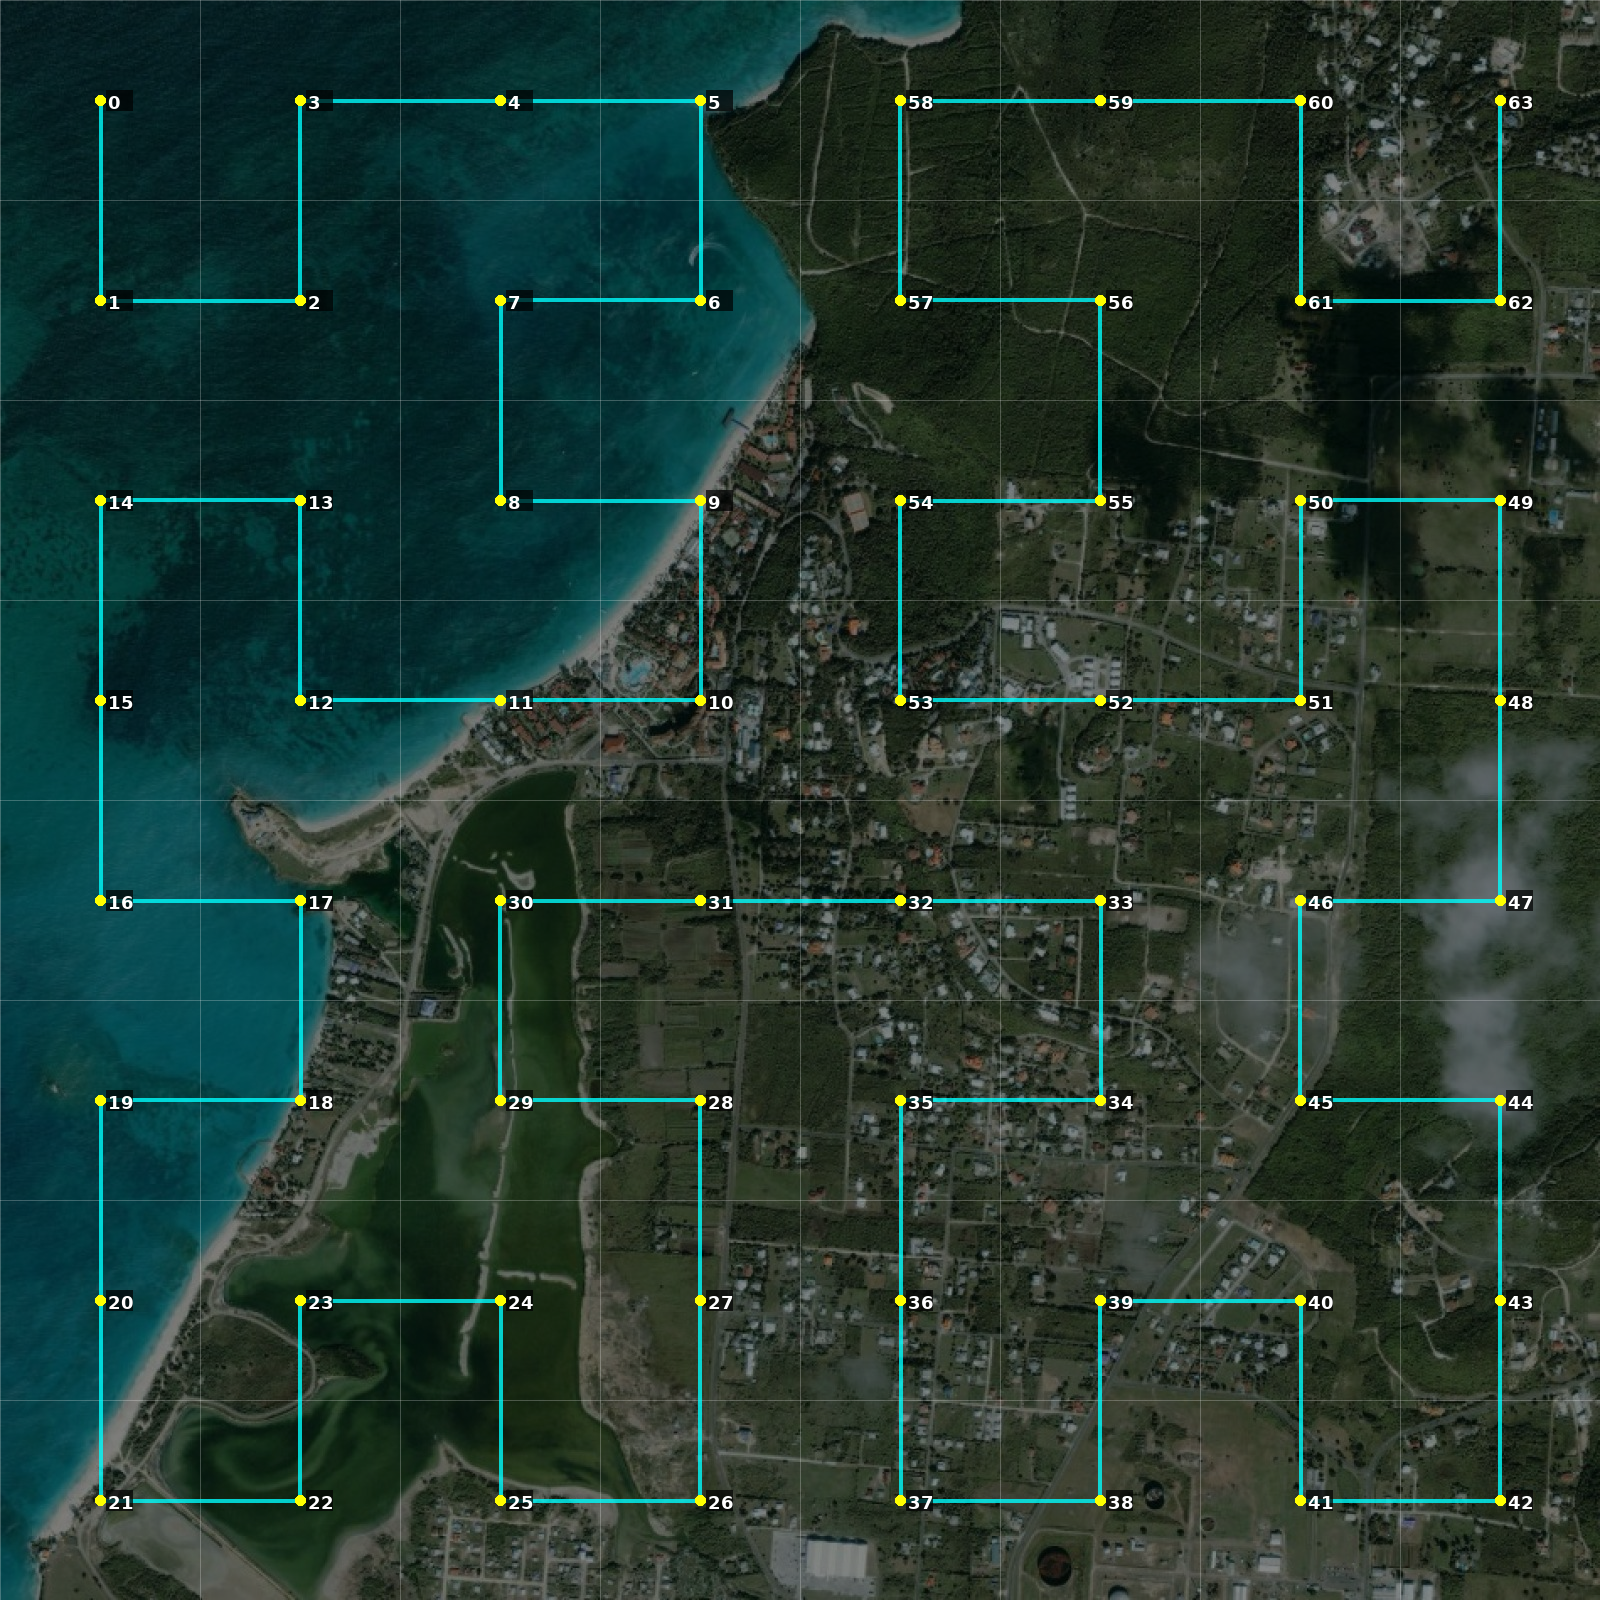
\includegraphics[width=\columnwidth]{hilbert_curve_visualization.png}
  \caption{Comparison of row-major (left) and Hilbert (right) indexing.
  Viewport codes are contiguous only under Hilbert ordering.}
  \label{fig:hilbert_vs_raster}
\end{figure}

\begin{figure*}[ht]
  \centering
  \begin{subfigure}[b]{0.24\textwidth}
    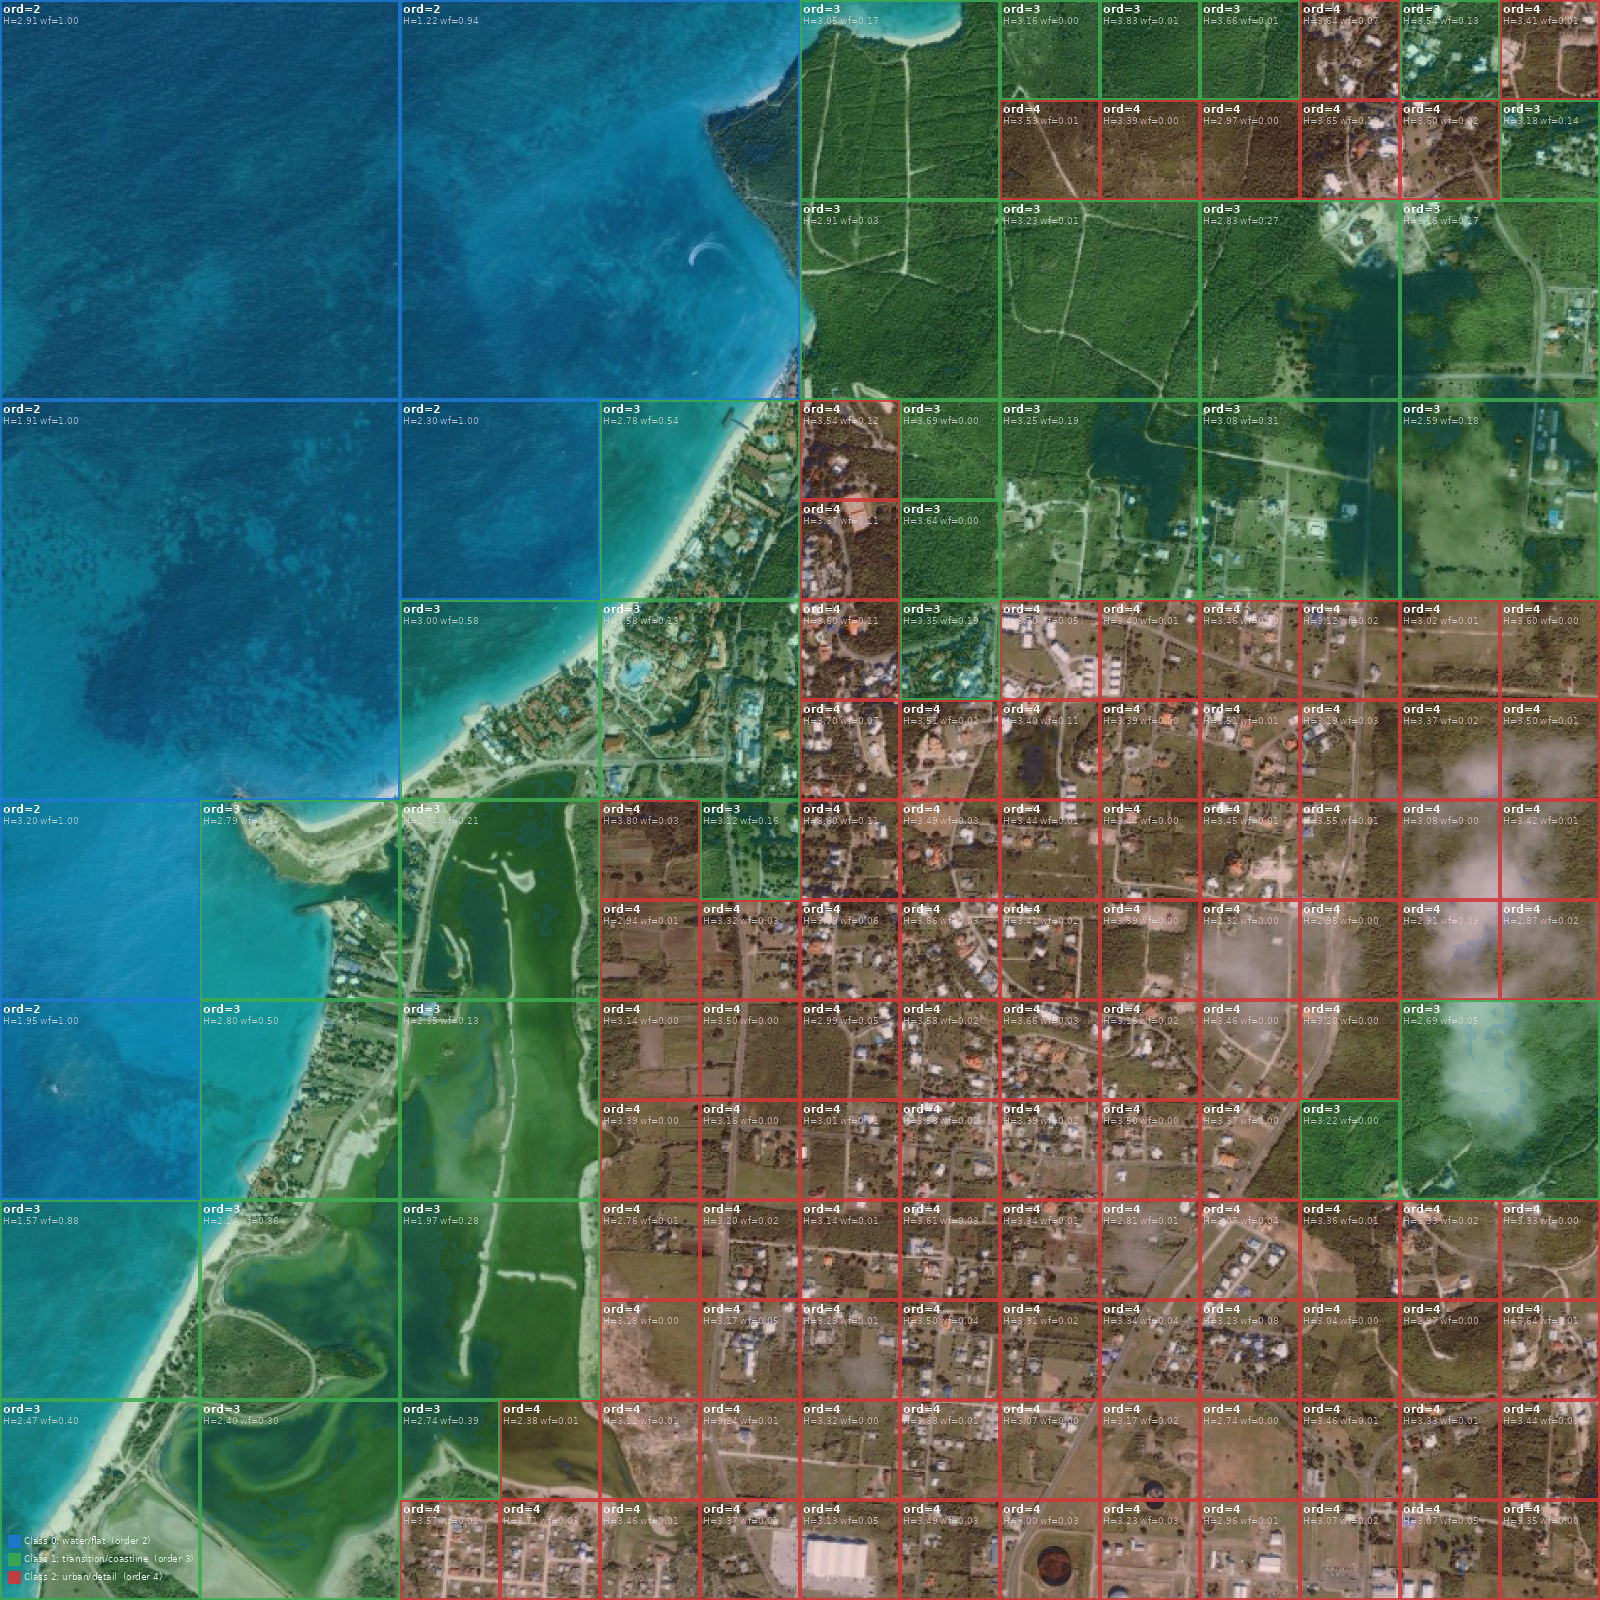
\includegraphics[width=\textwidth]{segmentation_vis.png}
    \caption{Segmentation by homogeneity and RGB values.}
    \label{fig:step_segmentation}
  \end{subfigure}\hfill
  \begin{subfigure}[b]{0.24\textwidth}
    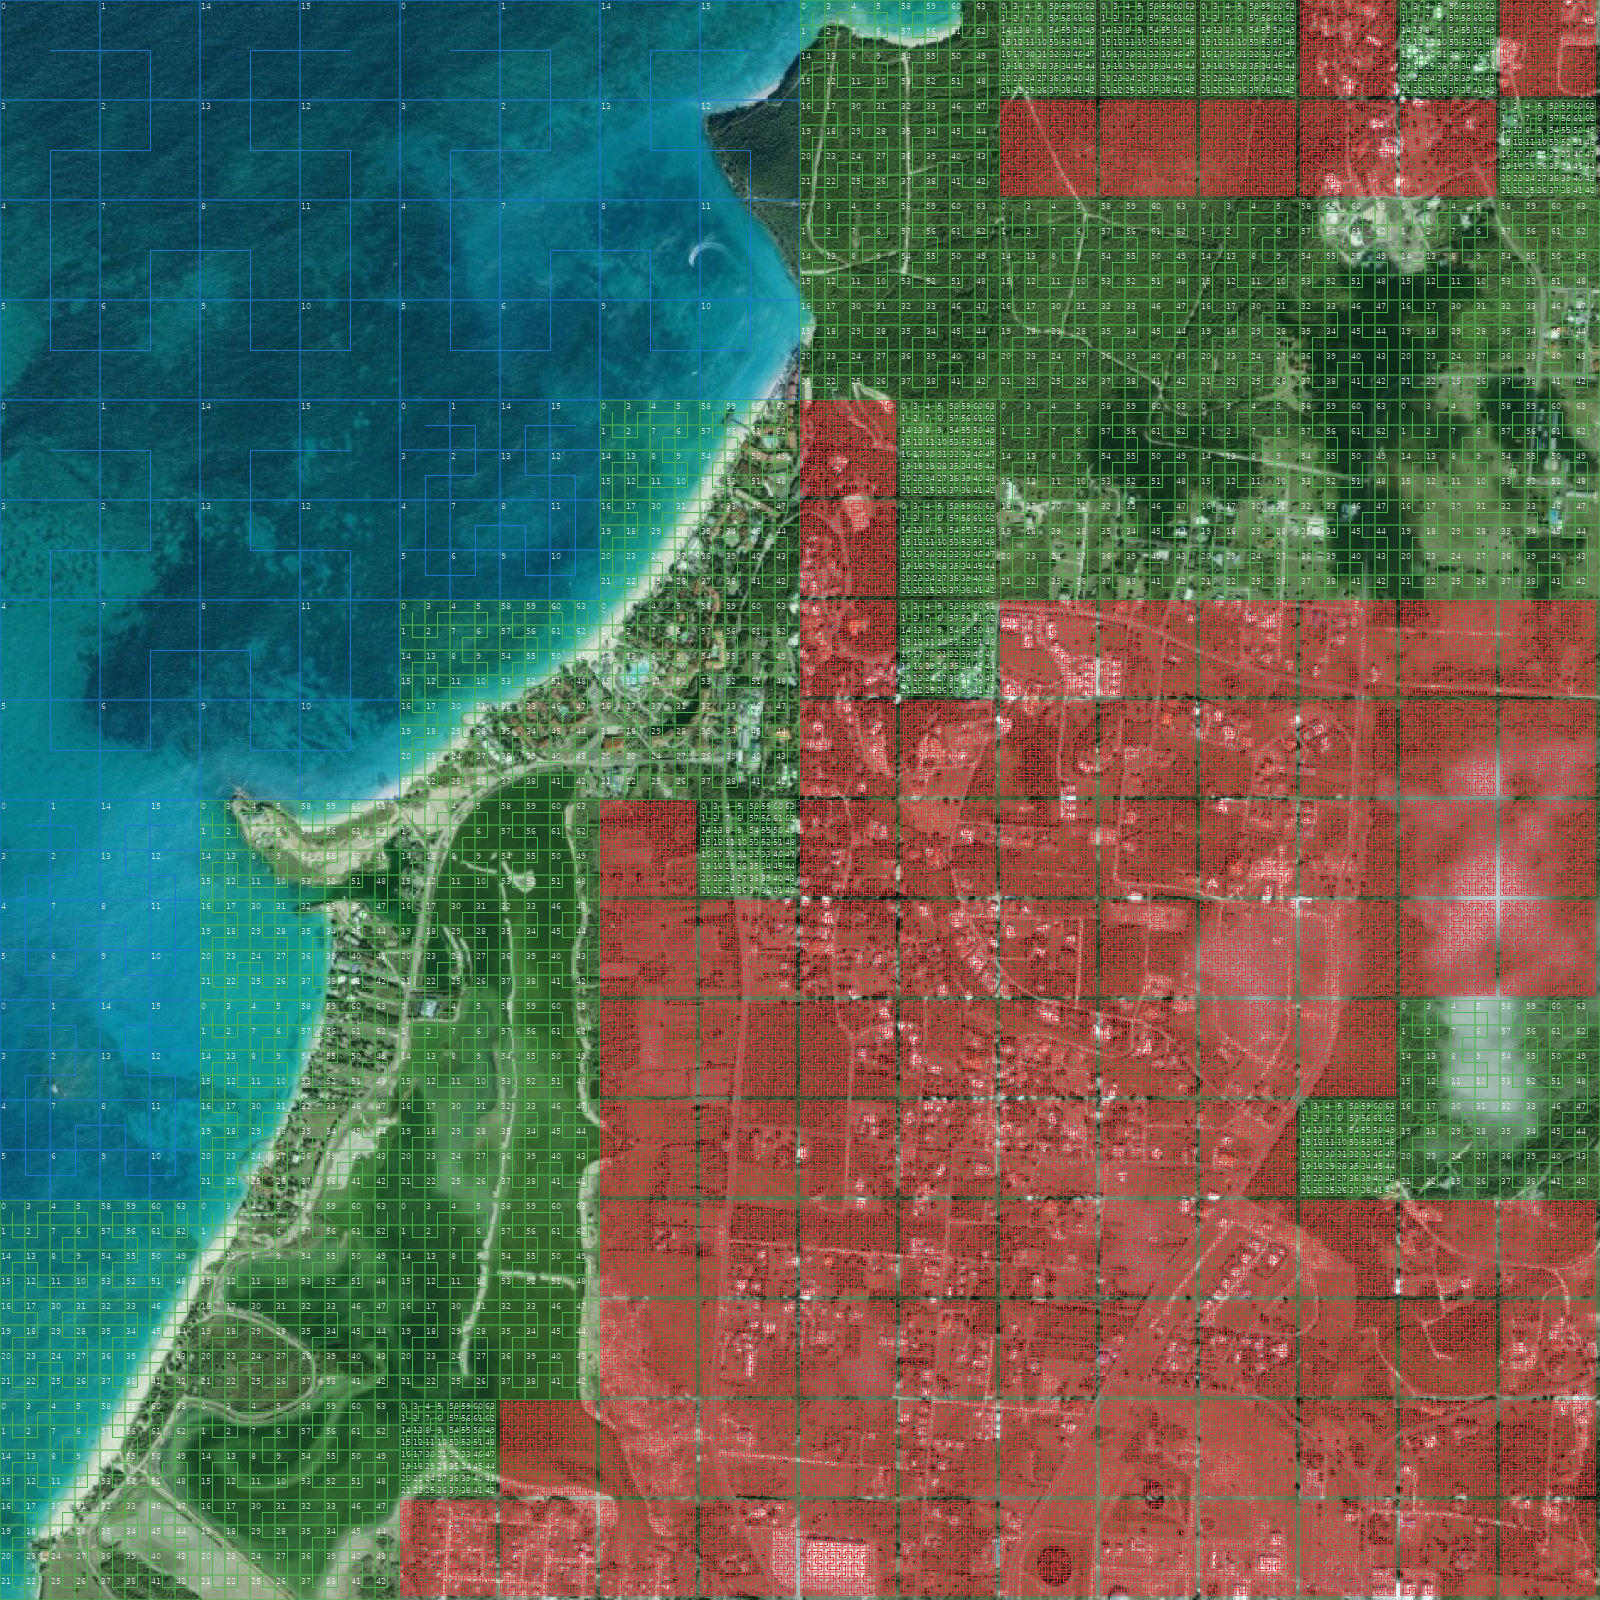
\includegraphics[width=\textwidth]{adaptive_hilbert_index_vis.png}
    \caption{Semantic Hilbert mapping per tile class.}
    \label{fig:step_semantic_hilbert}
  \end{subfigure}\hfill
  \begin{subfigure}[b]{0.24\textwidth}
    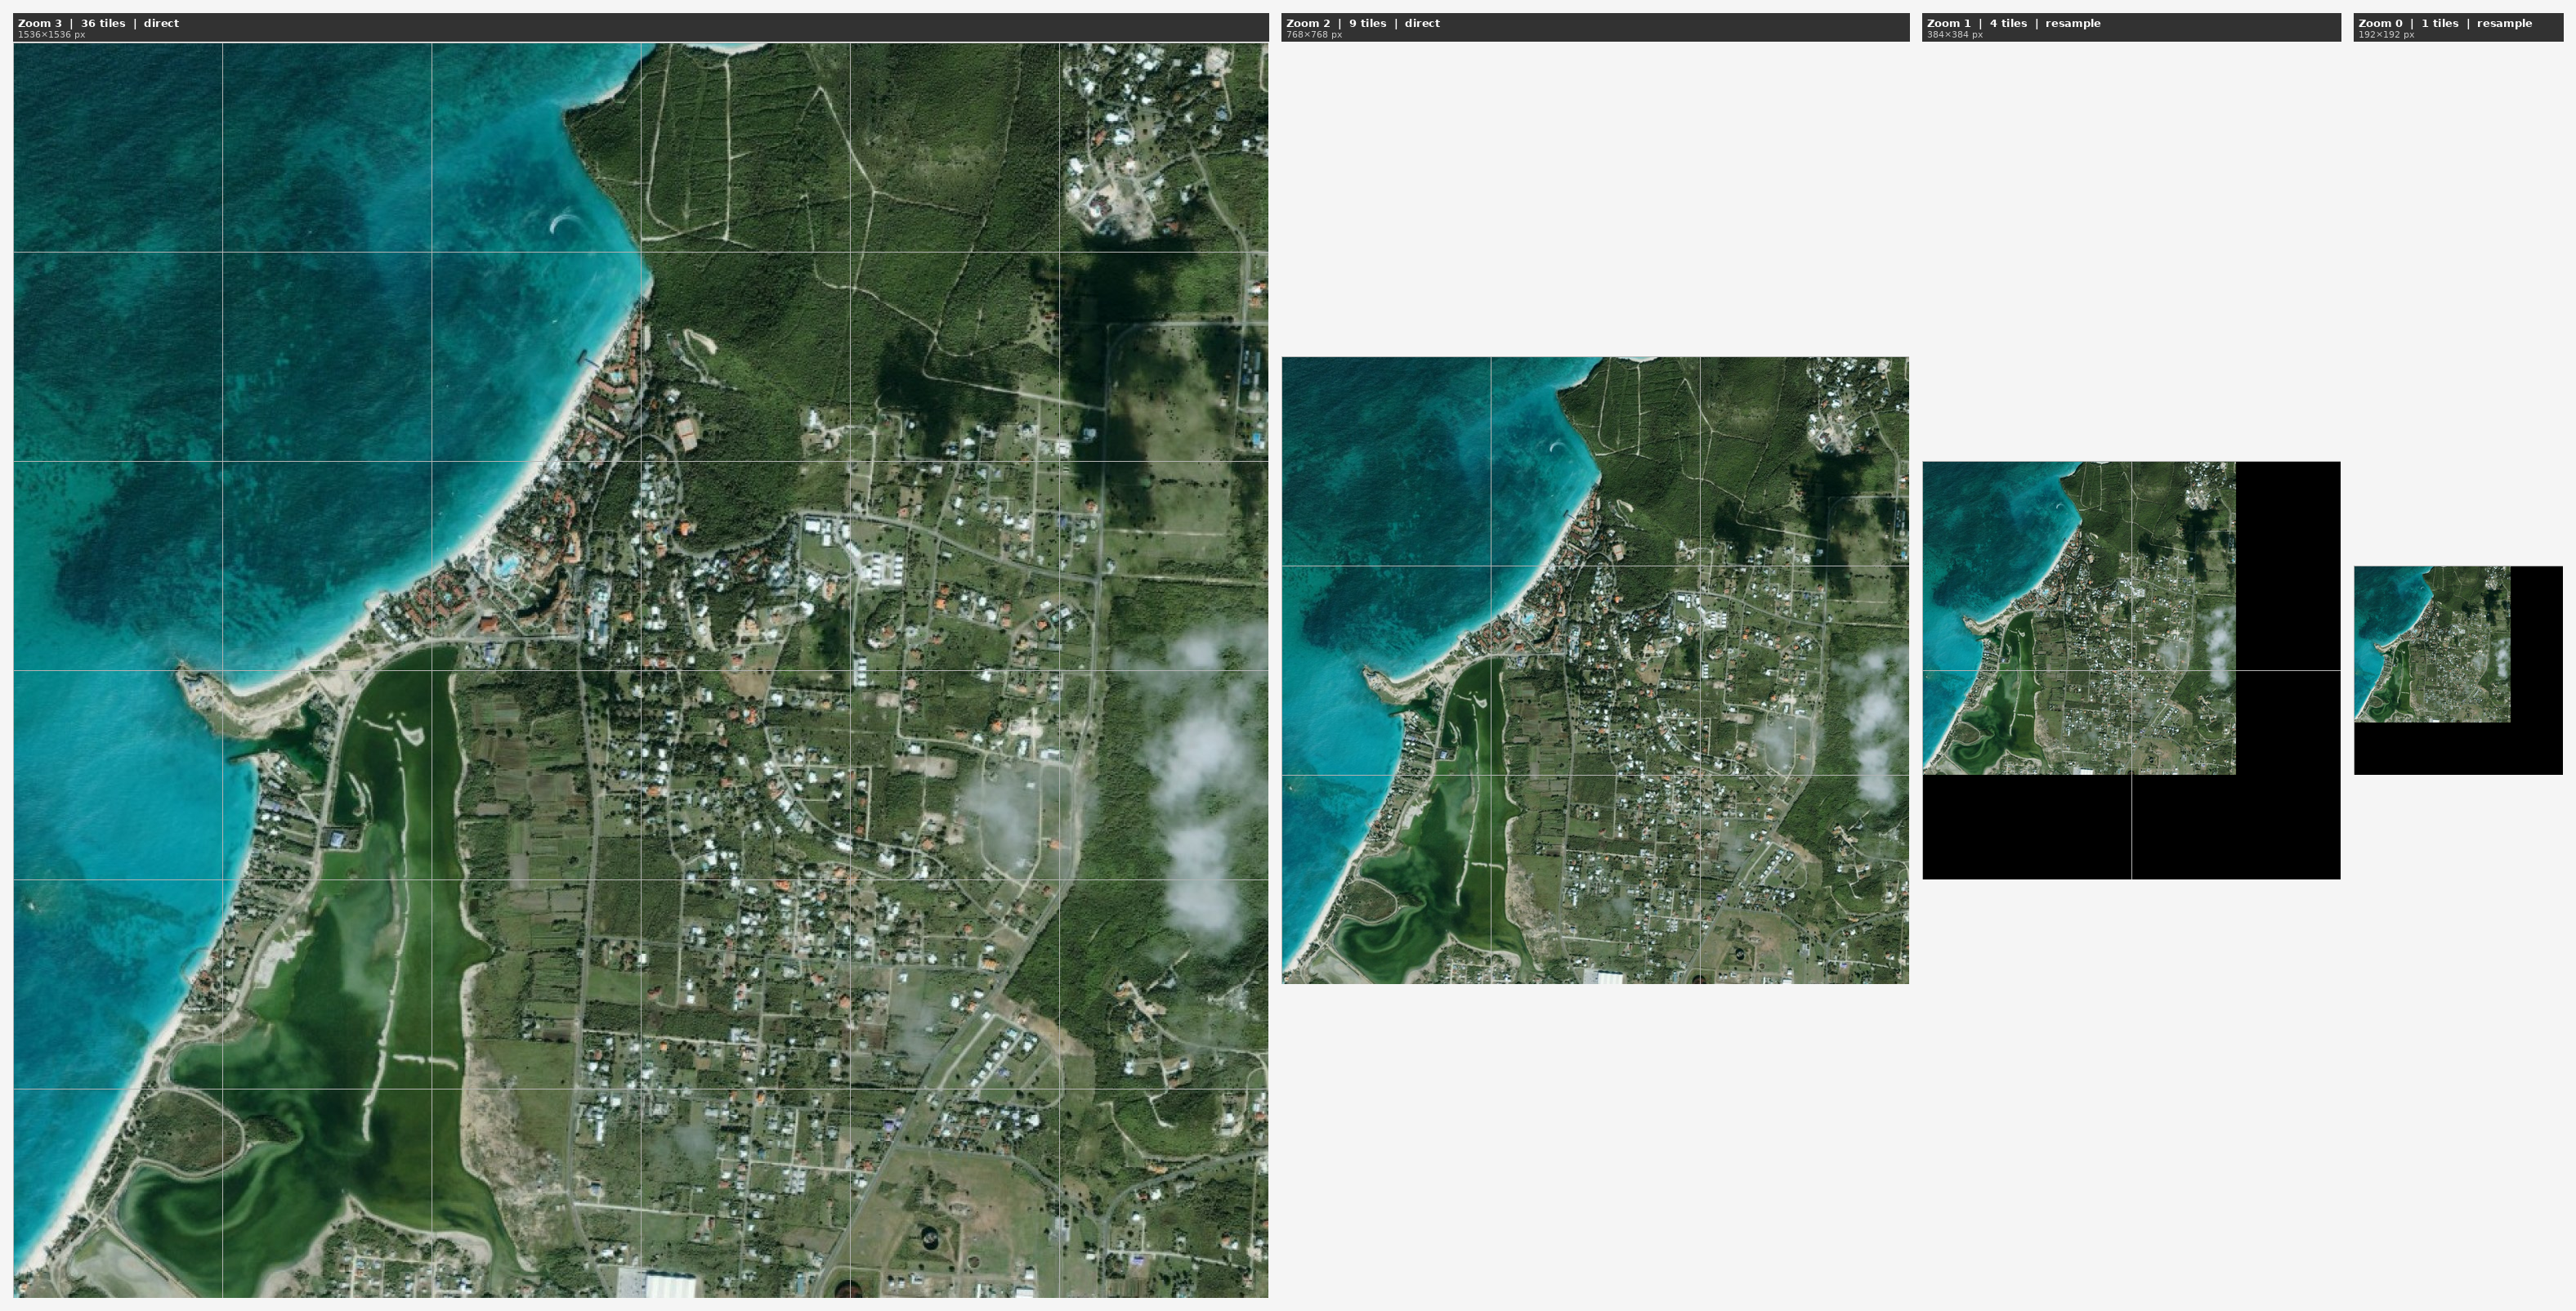
\includegraphics[width=\textwidth]{pyramid_summary_visualization.png}
    \caption{Adaptive Hilbert order across zoom levels.}
    \label{fig:step_hilbert_zoom}
  \end{subfigure}\hfill
  \begin{subfigure}[b]{0.24\textwidth}
    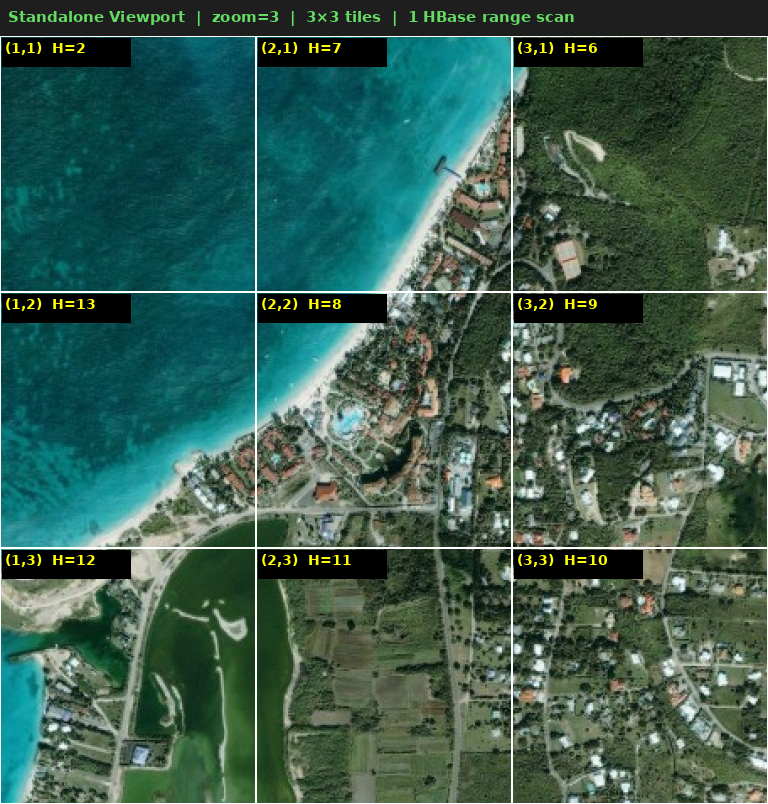
\includegraphics[width=\textwidth]{integration_standalone_view.png}
    \caption{Zoomed viewport rendering from the SAH display engine.}
    \label{fig:step_zoomed_view}
  \end{subfigure}
  \caption{End-to-end SAH processing pipeline: segmentation, semantic Hilbert order assignment, zoom-adaptive curve density, and final zoomed rendering.}
  \label{fig:pipeline_steps}
\end{figure*}

Fig.~\ref{fig:pipeline_steps} summarizes the processing stages in the SAH system: (a) initial segmentation based on tile homogeneity and RGB channel values, (b) semantic Hilbert mapping with class-dependent index order, (c) zoom-level adaptation of Hilbert curve density, and (d) the final rendered zoomed viewport.

\subsection{Tile Pyramid Construction}

Multi-resolution image tiles are generated directly from raw source raster files, bypassing the traditional mosaic $\to$ pyramid $\to$ tile pipeline.

\begin{itemize}
  \item \textbf{Fine zoom (level 3):} Tiles rendered directly from
intersecting source rasters.
  \item \textbf{Coarse zoom (levels 0--2):} Four child tiles downsampled via
bilinear resampling into a single parent tile.
\end{itemize}

The system generates 50 optimized tiles in approximately 1.16 seconds, eliminating the pre-mosaicking bottleneck entirely.

\subsection{RAM-Resident Data Structures}

At server startup, SAH builds four data structures loaded entirely into RAM. No disk reads occur during query serving.

\begin{enumerate}
  \item \textbf{R-Tree.} Spatial bounding-box index over all 145 base tiles.
Reduces 145 tile candidates to $\approx$8 in $\approx$7 comparisons, permanently pruning 137 tiles from all subsequent computations.
  \item \textbf{Hilbert Cache.} Precomputed lookup table that maps each
tile ID, row, and column tuple to its Hilbert code, enabling $O(1)$ range extraction.
  \item \textbf{Class Order Index.} A 31{,}072-record array sorted by Hilbert
code, with sub-tiles grouped by semantic class. This is the structure against which binary search (\texttt{bisect}) operates.
  \item \textbf{Base Lookup.} Direct coordinate-to-tile dictionary enabling
single-tile instantaneous retrieval without traversal.
\end{enumerate}

The query execution flow is: R-Tree $\to$ Hilbert Cache $\to$ Class Order Index $\to$ Base Lookup.

% ── IV. Query Engine ──────────────────────────────────────────────────────────
\section{Query Engine}

Every user interaction, whether pan, zoom, or click, triggers a deterministic four-step query sequence.

\textbf{Step 0: R-Tree Intersection.} The viewport bounding box is
submitted to the R-tree, reducing 145 tiles to $\approx$8 candidates. More than 107 tiles are pruned before any Hilbert computation begins.

\textbf{Step 1: Range Extraction.} Sub-cells within the viewport are
identified via the Hilbert Cache. The 2D spatial region is converted to a 1D numerical interval $[h_{\min},\, h_{\max}]$.

\textbf{Step 2: Range Merging.} Overlapping Hilbert code intervals are
sorted and merged into a minimal non-overlapping set, preventing redundant
\texttt{bisect} invocations.

\textbf{Step 3: Sorted Array Bisect.} Binary search locates $h_{\min}$ in
the Class Order Index and reads contiguously to $h_{\max}$. A final center-point membership check discards geometric false positives introduced by Hilbert curve boundary effects.

This sequence skips between 96\% and 99.9\% of all index records per query, depending on zoom depth.

% ── V. Performance Evaluation ─────────────────────────────────────────────────
\section{Performance Evaluation}

\subsection{Query Cost vs.\ Zoom Depth}

Table~\ref{tab:perf} presents query cost measurements across zoom levels on the 145-tile dataset containing 31{,}072 total index records.

\begin{table}[ht]
  \caption{Query Cost vs.\ Zoom Depth}
  \label{tab:perf}
  \centering
  \scriptsize
  \renewcommand{\arraystretch}{1.25}
  \begin{tabular}{C{0.75cm} L{1.65cm} C{1.15cm} C{1.15cm} C{1.2cm}}
    \toprule
    \textbf{Depth} & \textbf{Viewport} & \textbf{Hilbert Range} &
    \textbf{Examined} & \textbf{Skipped} \\
    \midrule
    0 & Full image        & $0 \to 255$     & 1{,}024 & $\sim$70\%   \\
    1 & $500\times500$    & $32 \to 223$    &     764 & $\sim$75\%   \\
    2 & 1/16 of image     & $80 \to 175$    &     380 & $\sim$88\%   \\
    3 & 1/64 of image     & $112 \to 143$   &     124 & $\sim$95\%   \\
    5 & 1/1024 of image   & $127 \to 134$   &      28 & $\sim$99.9\% \\
    \bottomrule
  \end{tabular}
\end{table}

A critical property of SAH is that query cost \textit{improves} as the viewport narrows. Unlike traditional quadtrees which degrade at deep zoom (more nodes require traversal), SAH benefits from narrower viewports because they map to smaller Hilbert code ranges. At depth 5, only 1 of 145 base tiles enters R-tree consideration, and computational cost approaches a constant regardless of total dataset size.

\subsection{Comparative Complexity Analysis}

Table~\ref{tab:compare} compares SAH against naive sequential scanning across key system dimensions. For a focused viewport query, the naive system scans all 31{,}072 records in $O(N)$ time, taking 22.28\,ms in benchmark conditions. SAH examines $\approx$42 records in $O(\log N + K)$ time, achieving a $214.2\times$ speedup. The performance gap widens proportionally as the dataset grows, since $K \ll N$ at any realistic zoom level.

\begin{table}[t]
  \caption{SAH vs.\ Legacy System Comparison}
  \label{tab:compare}
  \centering
  \scriptsize
  \renewcommand{\arraystretch}{1.1}
  \setlength{\tabcolsep}{3pt}
  \begin{tabular}{l c c}
    \toprule
    \textbf{Metric} & \textbf{Legacy} & \textbf{SAH} \\
    \midrule
    Grid Structure & Uniform & Content-aware \\
    Indexing Logic & Row-major & Hilbert + binary search \\
    Empty Space & Uniformly processed & Skipped entirely \\
    Display Support & Single target & Unified distributed \\
    Search Complexity & $O(N)$ & $O(\log N + K)$ \\
    Peak Speedup & N/A & $\mathbf{56\times}$ faster \\
    \bottomrule
  \end{tabular}
\end{table}

% ── VI. Dual Display Support ──────────────────────────────────────────────────
\section{Dual Display Support}

The SAH backend serves two fundamentally different rendering targets without architectural modification.

\textbf{Condition A: Standalone Display.} A React canvas frontend paired
with a Flask tile server. A $3\times3$ viewport window is retrieved in 0.014\,ms at a 75\% cache hit rate. Collapsed tiles (outside the active viewport) are rendered as solid-color rectangles, preserving local RAM.

\textbf{Condition B: Distributed SAGE2 Wall.} An 8-panel $7680\times2160$
distributed display wall. The 8-panel wall synchronizes within approximately 17\,ms, within the 33\,ms budget imposed by 30\,fps rendering. The Hilbert curve property that adjacent regions share contiguous code ranges ensures that adjacent display panels receive contiguous code intervals, guaranteeing seamless stitching with zero content gaps or overlaps. (Figure \ref{fig:sage2_wall})

\begin{figure}[!t]
  \centering
  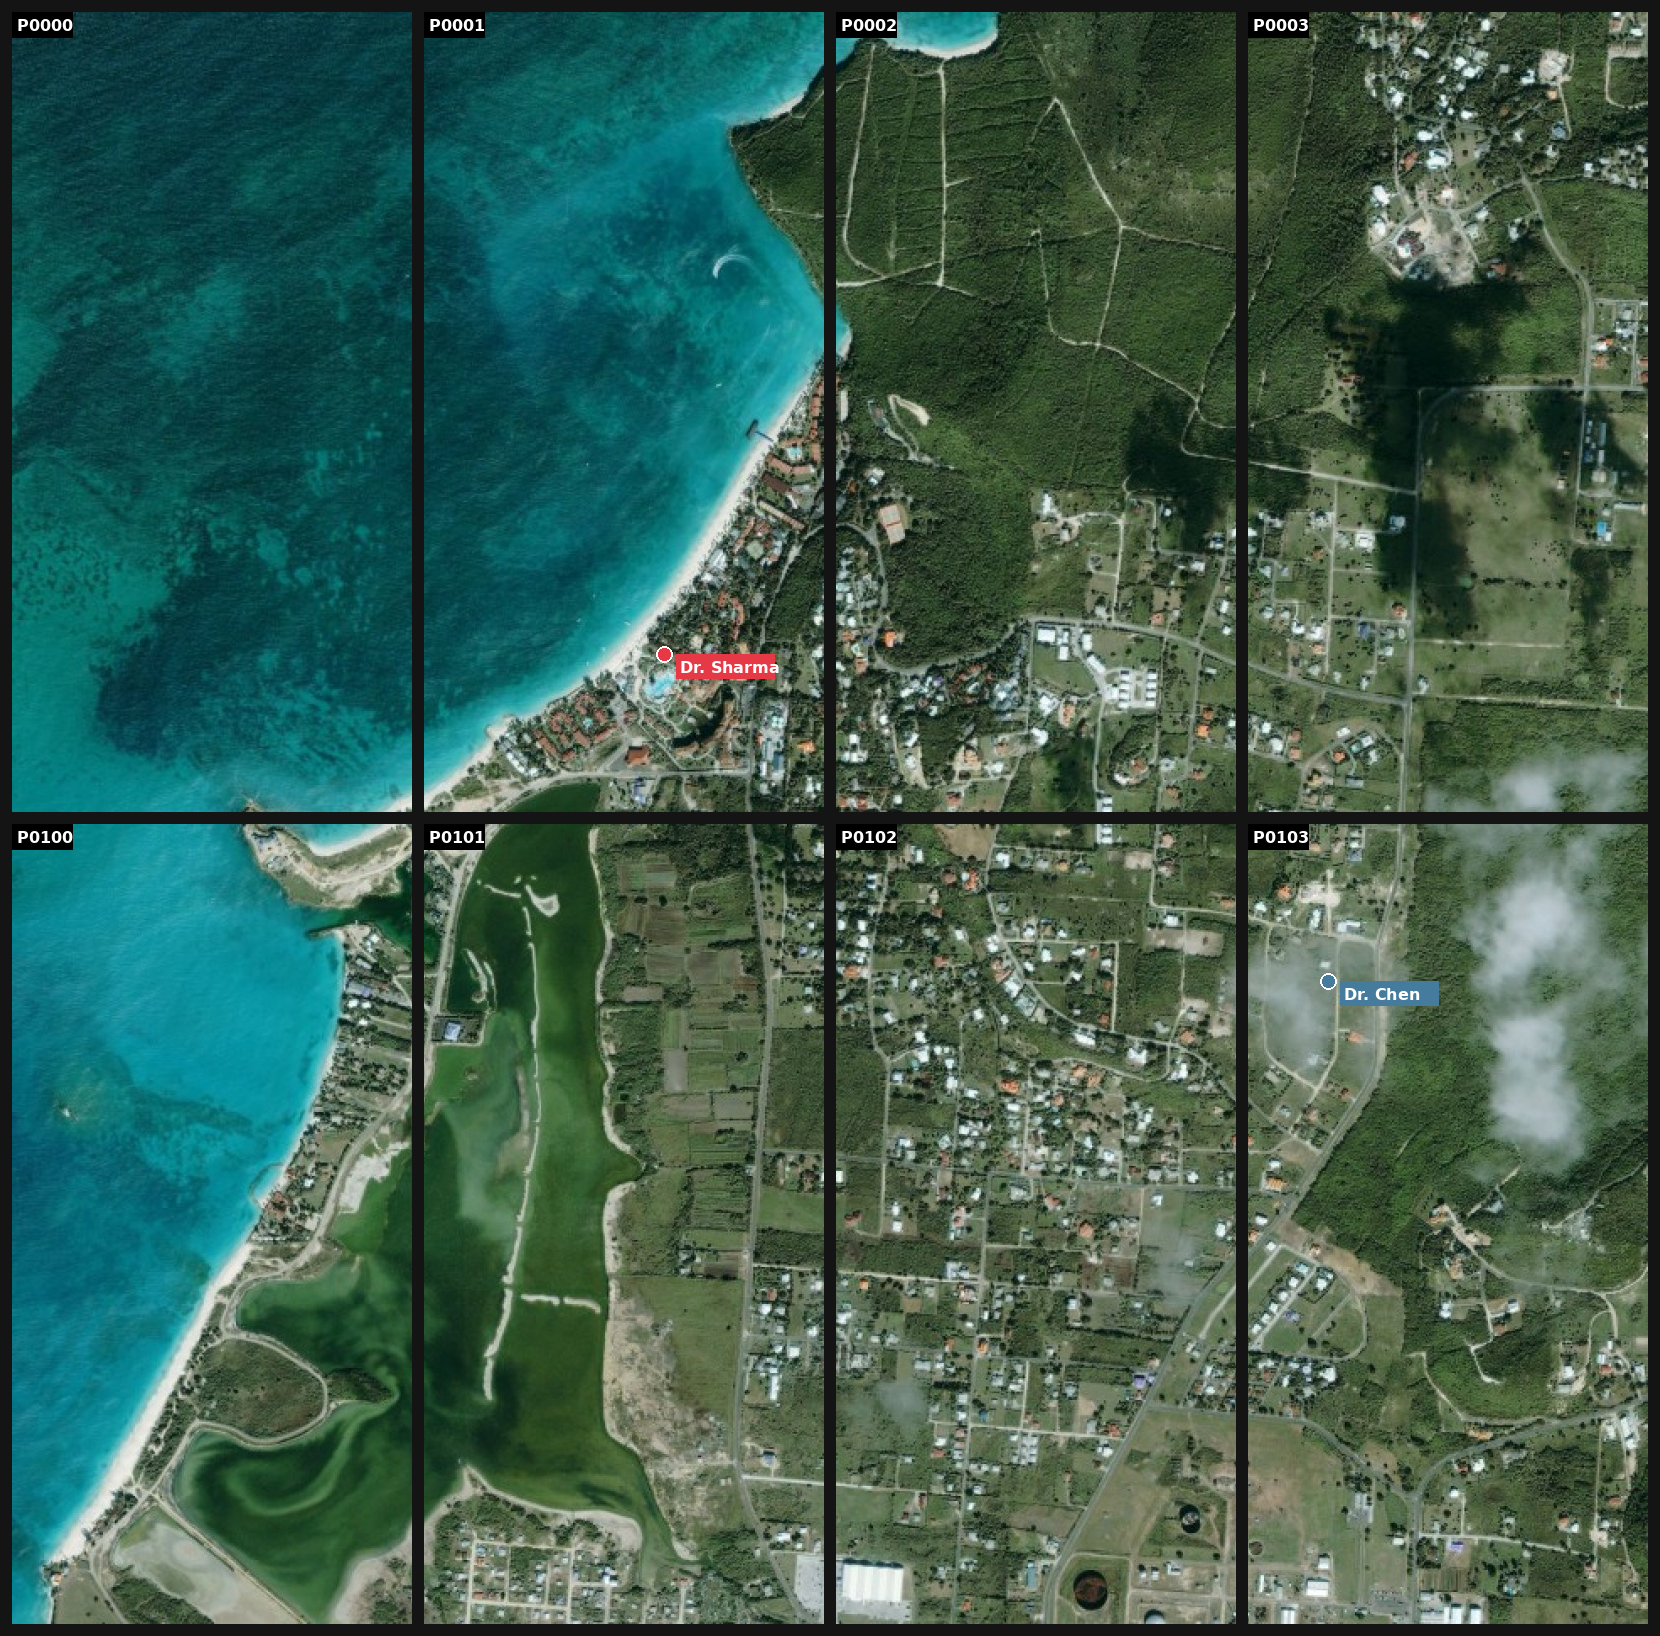
\includegraphics[width=\columnwidth]{sage2_display_wall_sim.png}
  \caption{SAGE2 distributed 8-panel display wall rendering a zoomed viewport with SAH backend serving seamlessly across all panels without modification.}
  \label{fig:sage2_wall}
\end{figure}

% ── VII. Display Order vs. Index Order ────────────────────────────────────────
\section{Display Order vs.\ Index Order Distinction}

Each base tile carries two completely independent Hilbert orders that must not be conflated.

\textbf{Base Index Order} is fixed at build time and determined by Shannon
entropy. It controls how many sub-cells exist in the sorted array for query purposes and never changes regardless of zoom level:
\begin{itemize}
  \item Water $\to$ Order 2 $\to$ 16 cells (codes 0--15)
  \item Coast $\to$ Order 3 $\to$ 64 cells (codes 0--63)
  \item Urban $\to$ Order 4 $\to$ 256 cells (codes 0--255)
\end{itemize}

\begin{figure*}[!t]
  \centering
  \begin{subfigure}[b]{0.24\textwidth}
    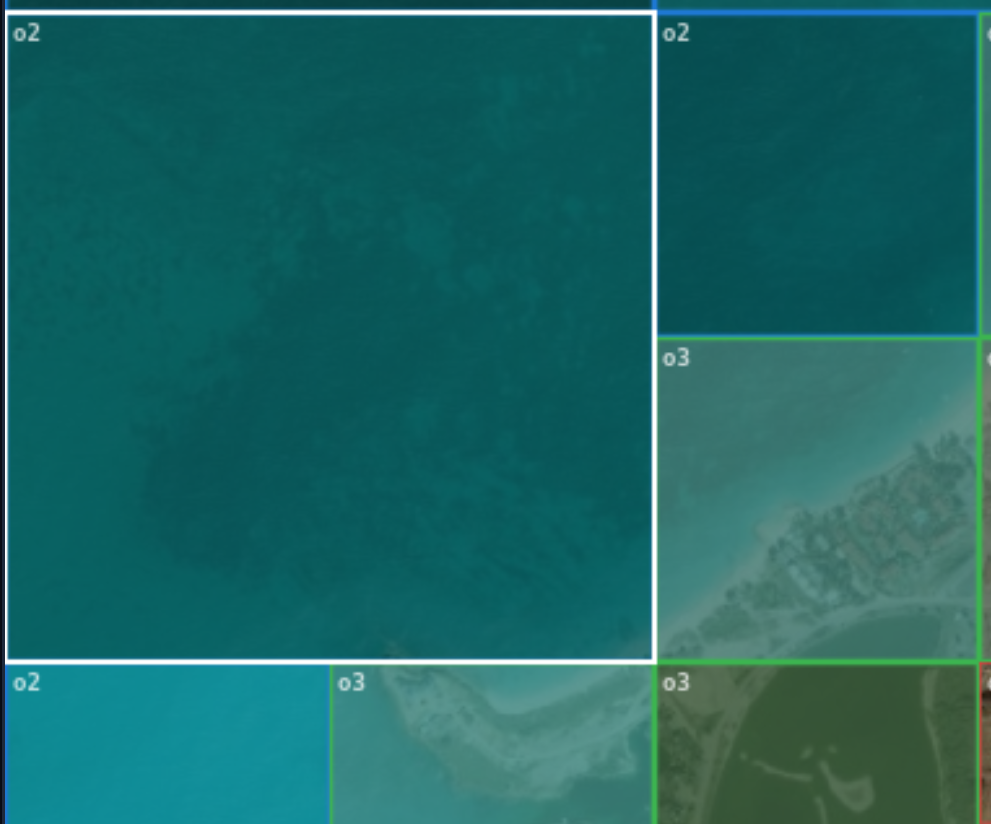
\includegraphics[width=\textwidth]{zoom0.png}
    \caption{Zoom level 0}
    \label{fig:zoom0}
  \end{subfigure}\hfill
  \begin{subfigure}[b]{0.24\textwidth}
    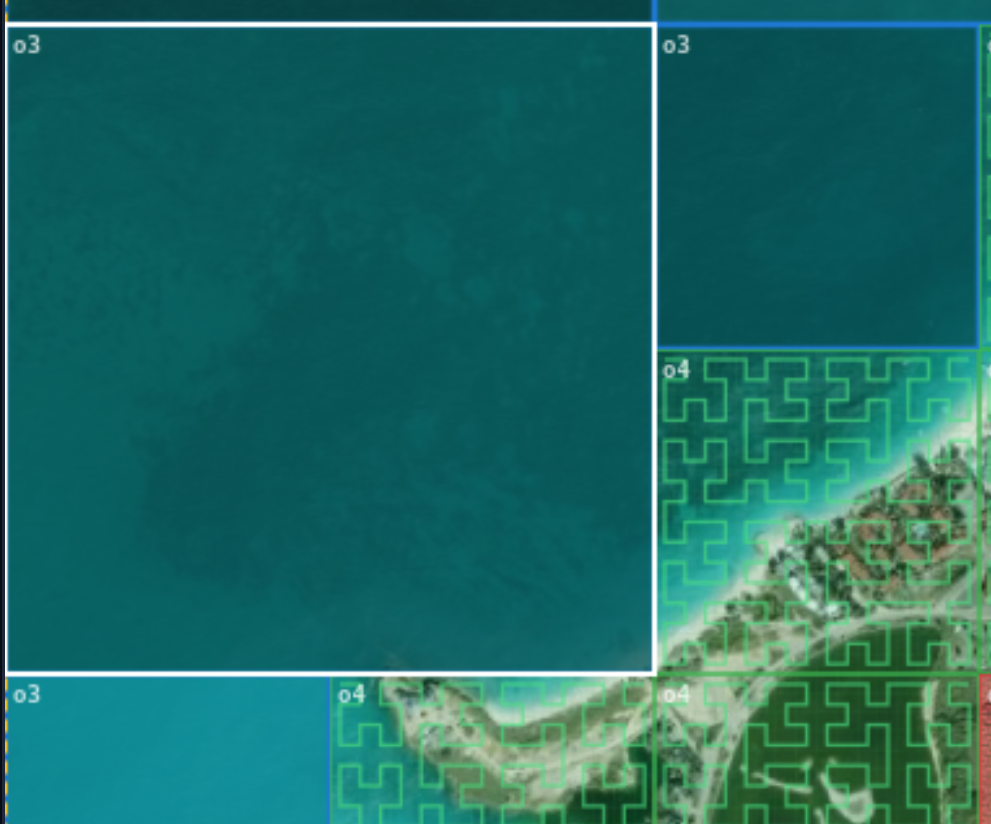
\includegraphics[width=\textwidth]{zoom1.png}
    \caption{Zoom level 1}
    \label{fig:zoom1}
  \end{subfigure}\hfill
  \begin{subfigure}[b]{0.24\textwidth}
    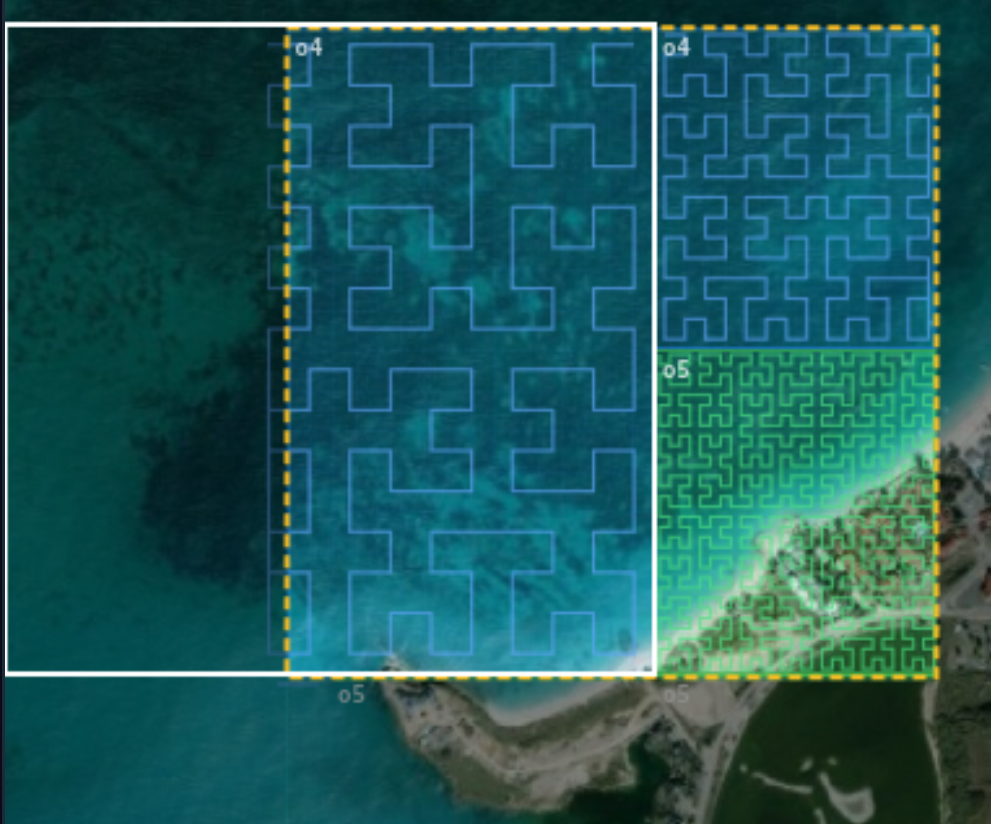
\includegraphics[width=\textwidth]{zoom2.png}
    \caption{Zoom level 2}
    \label{fig:zoom2}
  \end{subfigure}\hfill
  \begin{subfigure}[b]{0.24\textwidth}
    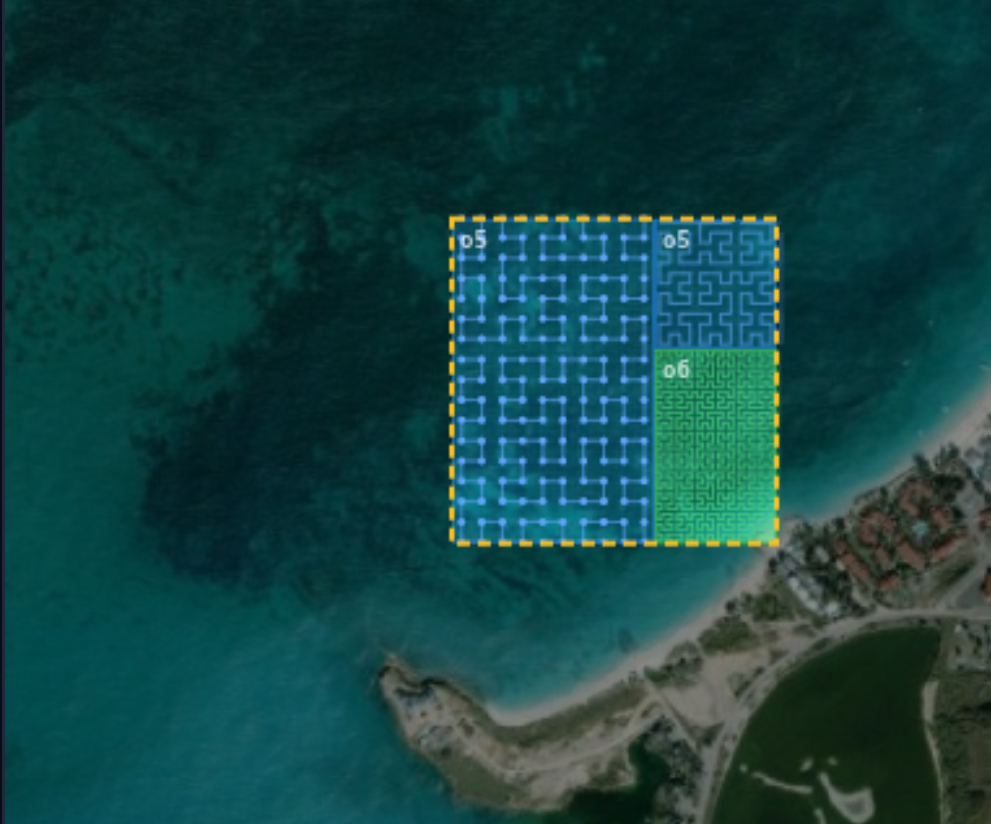
\includegraphics[width=\textwidth]{zoom3.png}
    \caption{Zoom level 3}
    \label{fig:zoom3}
  \end{subfigure}
  \caption{Zoom-dependent visual Hilbert order for a single tile across display levels 0--3. The index order is fixed, but the rendered curve density increases with zoom.}
  \label{fig:zoom_levels}
\end{figure*}

\textbf{Display Render Order} is computed fresh at each zoom level and never
stored. It controls the visual density of the Hilbert curve drawn on canvas and is computed as:
\begin{equation}
  d_{\text{display}} = d_{\text{base}} + z_{\text{current}}
  \label{eq:displayorder}
\end{equation}
Fig.~\ref{fig:zoom_levels} shows the same tile rendered at zoom levels 0--3, where the visible Hilbert curve becomes denser even though the base index order remains fixed.

where $z_{\text{current}}$ is the current zoom depth. For example, a water tile at depth 3 draws an order-5 visual curve on screen while the query engine still bisects against 16 cells with codes 0--15. The visual curve growing denser as the user zooms is purely cosmetic; the index curve never changes.

% ── VIII. Discussion ─────────────────────────────────────────────────────────
\section{Discussion}

\subsection{Raster vs.\ Vector Implementation}
The raster pipeline generates multi-resolution image tiles directly from raw source files without a mosaicking step and assigns Hilbert codes to pixel sub-cells. The vector pipeline groups features such as LineStrings into Hilbert sub-grids by spatial centroid and stores them in a JSON index. In future work, the main differences could include:
\begin{itemize}
  \item \textbf{Progressive Loading:} Vector data can be simplified dynamically based on zoom level (Level of Detail) to prevent rendering overly complex paths when zoomed out, whereas raster data primarily involves rendering pre-computed downsampled parent tiles.
  \item \textbf{Data Streaming:} Raster data sends rendered image tiles to the frontend, while vector data streams geometric coordinates to the client for on-the-fly rendering and styling.
\end{itemize}

\subsection{Fairness of Baseline Comparison}
The comparison between SAH and the ``Legacy Naive Scan'' is inherently unfair, as the legacy system uses an $O(N)$ row-major scan over all records, processing empty space uniformly. Comparing an indexed approach (SAH) to a completely unindexed scan exaggerates the performance gain. To make the comparison fair, the baseline should use a standard spatial index, such as an R-Tree or a uniform Quadtree, over the entire dataset. This would isolate the performance benefits specifically gained from the semantic-adaptive aspect and the Hilbert curve's spatial clustering.

\subsection{Multispectral (3-Band) Inputs}
Using a 3-band (RGB) or multispectral raster as input is highly beneficial. Shannon entropy and K-means heuristics can misclassify ambiguous zones, such as shallow water appearing as land. Richer feature information improves the accuracy of semantic classification (or future DeepLabV3 segmentation). The output index structure would remain identical, but the underlying tiles generated and served to the client would be RGB images rather than single-band maps, providing superior visual context.

\subsection{Memory Management and I/O}
High-memory files currently cause Out-Of-Memory errors because the architecture is 100\% RAM-resident with zero disk I/O, loading the entire sorted array at server startup. To save RAM and utilize I/O efficiently, the system can:
\begin{itemize}
  \item \textbf{Memory Mapping (mmap):} Map the large sorted index file to virtual memory instead of loading it entirely. The OS handles paging, pulling queried Hilbert ranges into RAM dynamically.
  \item \textbf{On-Disk Key-Value Stores:} Use a storage engine optimized for range queries (e.g., RocksDB). The \texttt{bisect} operation would perform disk seeks rather than consuming pure RAM.
  \item \textbf{Hierarchical Caching:} Keep only the R-Tree and Hilbert Cache in RAM, streaming sub-cell records from disk strictly on-demand.
\end{itemize}

\subsection{Large Vector Path Loading}
Loading the entire path for a massive vector file (e.g., a long highway) is highly inefficient at deep zoom levels. Better approaches include:
\begin{itemize}
  \item \textbf{Geometry Segmentation (Clipping):} Split long line paths into smaller segments at the boundaries of Hilbert sub-cells. This ensures a query only retrieves segments that physically intersect the current viewport.
  \item \textbf{Level of Detail (LoD):} For zoomed-out views, serve a simplified version of the path (using algorithms like Douglas-Peucker) to drastically reduce the number of vertices.
  \item \textbf{Vector Tiling:} Pre-generate vector tiles (e.g., Mapbox Vector Tiles) which inherently handle both segmentation and simplification across zoom levels.
\end{itemize}

% ── IX. Limitations ────────────────────────────────────────────────────────
\section{Limitations}

\textbf{Classification Accuracy.} Shannon entropy and water score heuristics
can misclassify ambiguous zones. Shallow water that appears land-colored (high red reflectance) is the primary failure case, as its water score may fall below the positive threshold despite being an aquatic region.

\textbf{Density Disadvantage.} SAH provides maximal benefit when the dataset
contains a mix of high- and low-complexity regions. In pathological cases where all tiles are uniformly dense ($H > 2.5$ everywhere), the Hilbert computation overhead produces a small performance penalty versus naive scanning.

\textbf{Incremental Updates.} The offline indexing pipeline requires a full
re-run to ingest new data. Targeted sub-region updates that preserve the existing index structure are not yet supported.

% ── X. Roadmap ───────────────────────────────────────────────────────────────
\section{Roadmap}

\textbf{Parallel Ingestion.} 32-core parallel processing for the indexing
pipeline, targeting a 20--30$\times$ reduction in pre-processing time for large datasets.

\textbf{Deep Learning Segmentation.} Replacement of the Shannon entropy
heuristic classifier with a DeepLabV3 semantic segmentation model~\cite{li2021quadtree}. This eliminates misclassification at ambiguous water--land boundaries and enables finer-grained class distinctions beyond the current three-class scheme.

\textbf{Alternative Space-Filling Encodings.} Investigation of alternative
space-filling encodings, including W-Hilbert~\cite{zhang2022whilbert} and fractal variants~\cite{rosso2020texture}, to determine whether any scheme outperforms the standard Hilbert curve in locality preservation for geospatial tile distributions.

% ── XI. Conclusion ─────────────────────────────────────────────────────────────
\section{Conclusion}

This work demonstrates that semantic awareness in spatial indexing produces compounding performance gains. By allocating index depth proportionally to visual complexity rather than uniformly, SAH reduces index size, eliminates empty-region waste, and enables binary-search query serving entirely in RAM. The Hilbert curve encoding ensures that spatial locality is preserved in the one-dimensional key space, directly enabling viewport queries to map to minimal contiguous index ranges.

The benchmark results, including a $214.2\times$ peak speedup, 99.9\% record pruning at depth 5, and sub-millisecond viewport retrieval, confirm that content-aware spatial indexing is a practically viable and highly effective alternative to uniform grid decomposition for heterogeneous geospatial raster datasets. The unified backend architecture supporting both standalone and distributed display targets without modification further demonstrates the generality of the SAH approach beyond single-display use cases.

\begin{thebibliography}{00}
  \bibitem{zhang2022whilbert} Lei, Yi & Tong, Xiaochong & Wang, Dali & Qiu, Chunping & Li, He & Zhang, Youwei. (2023). W-Hilbert: A W-shaped Hilbert curve and coding method for multiscale geospatial data index. International Journal of Applied Earth Observation and Geoinformation. 118. 103298. 10.1016/j.jag.2023.103298. 

  \bibitem{li2021quadtree} Zhang, Hua & Jiang, Zhengang & Zheng, Guoxun & Yao, Xuekun. (2023). Semantic Segmentation of High-Resolution Remote Sensing Images with Improved U-Net Based on Transfer Learning. International Journal of Computational Intelligence Systems. 16. 10.1007/s44196-023-00364-w. 

  \bibitem{rosso2020texture} Casanova, Dalcimar & Florindo, João & Falvo, Mauricio. (2016). Texture analysis using fractal descriptors estimated by the mutual interference of color channels. Information Sciences. 346. 10.1016/j.ins.2016.01.077. 

  \bibitem{bariviera2024texture} Bariviera, Aurelio F. & Hansen, Roberta & Pastor, Verónica. (2024). Texture Discrimination via Hilbert Curve Path Based Information Quantifiers. 10.48550/arXiv.2409.15327. 

  \bibitem{lawder2001querying} Lawder, Jonathan & King, Peter. (2001). Querying Multi-dimensional Data Indexed Using the Hilbert Space-filling Curve.. SIGMOD Record. 30. 19-24. 10.1145/373626.373678. 
  
\end{thebibliography}

\end{document}
